\chapter{Flight Strategy and Obstacle Avoidance}
	
	This chapter describes the proposed and implemented flight strategy, including the obstacle avoidance technique. Now that stable flight has been achieved a more advanced flight routine can be implemented. The chapter begins by describing the proposed flight strategy for missions in a narrow corridor and confined space. After the flight strategy has been discussed, an obstacle avoidance routine is proposed and implemented. The obstacle avoidance methodology is discussed, including sensor placement and continues on to describe the mathematical modelling of the environment and the sensors for use in the simulation. Once the modelling is adequate, the avoidance controller design is described and is followed by the testing of the routine. The obstacle avoidance routine is based on proximity measurements to the aircraft's immediate surroundings.
	
	\section{Flight Strategy}
	This section describes the flight strategy proposed for flight inside a confined narrow corridor. The first step to creating a mission will be to implement a waypoint generator, allowing for mission locations to be preloaded into the craft and followed sequentially. The platform design has been previously discussed and was chosen to be a narrow, elongated design. For an aircraft of this design it is deemed beneficial for constant yaw alignment as it traverses down the corridor. The section first describes the waypoint generator proceeded by the strategy for yaw alignment.
	
		\subsection{Waypoint Generation}
		The waypoint generator is implemented as a buffer of North, East and Down position references. The references are preloaded into the drone at mission start through a ground station. Once a mission is begun the set points are fed into the relevant position controllers. Although not required, it is suggested that the first waypoint is always the starting North East location with a desired altitude reference. This allows the drone to first reach a desired height before continuing the mission.
		
		The ground station can program an acceptable position error limit for each waypoint. Once the limit in all three axes is reached, the waypoint generator begins a timer which, when lapses, steps on to the next waypoint in the list. The ground station also has the option to move onto the next waypoint prematurely if desired.
		
		Figure \ref{IM_WaypointFlight} shows a simple followed flight path set up by the waypoint generator. The blue line shown is the flown path, while the cyan dots represent the waypoints.
		
		\begin{figure}[H]
			\centering
			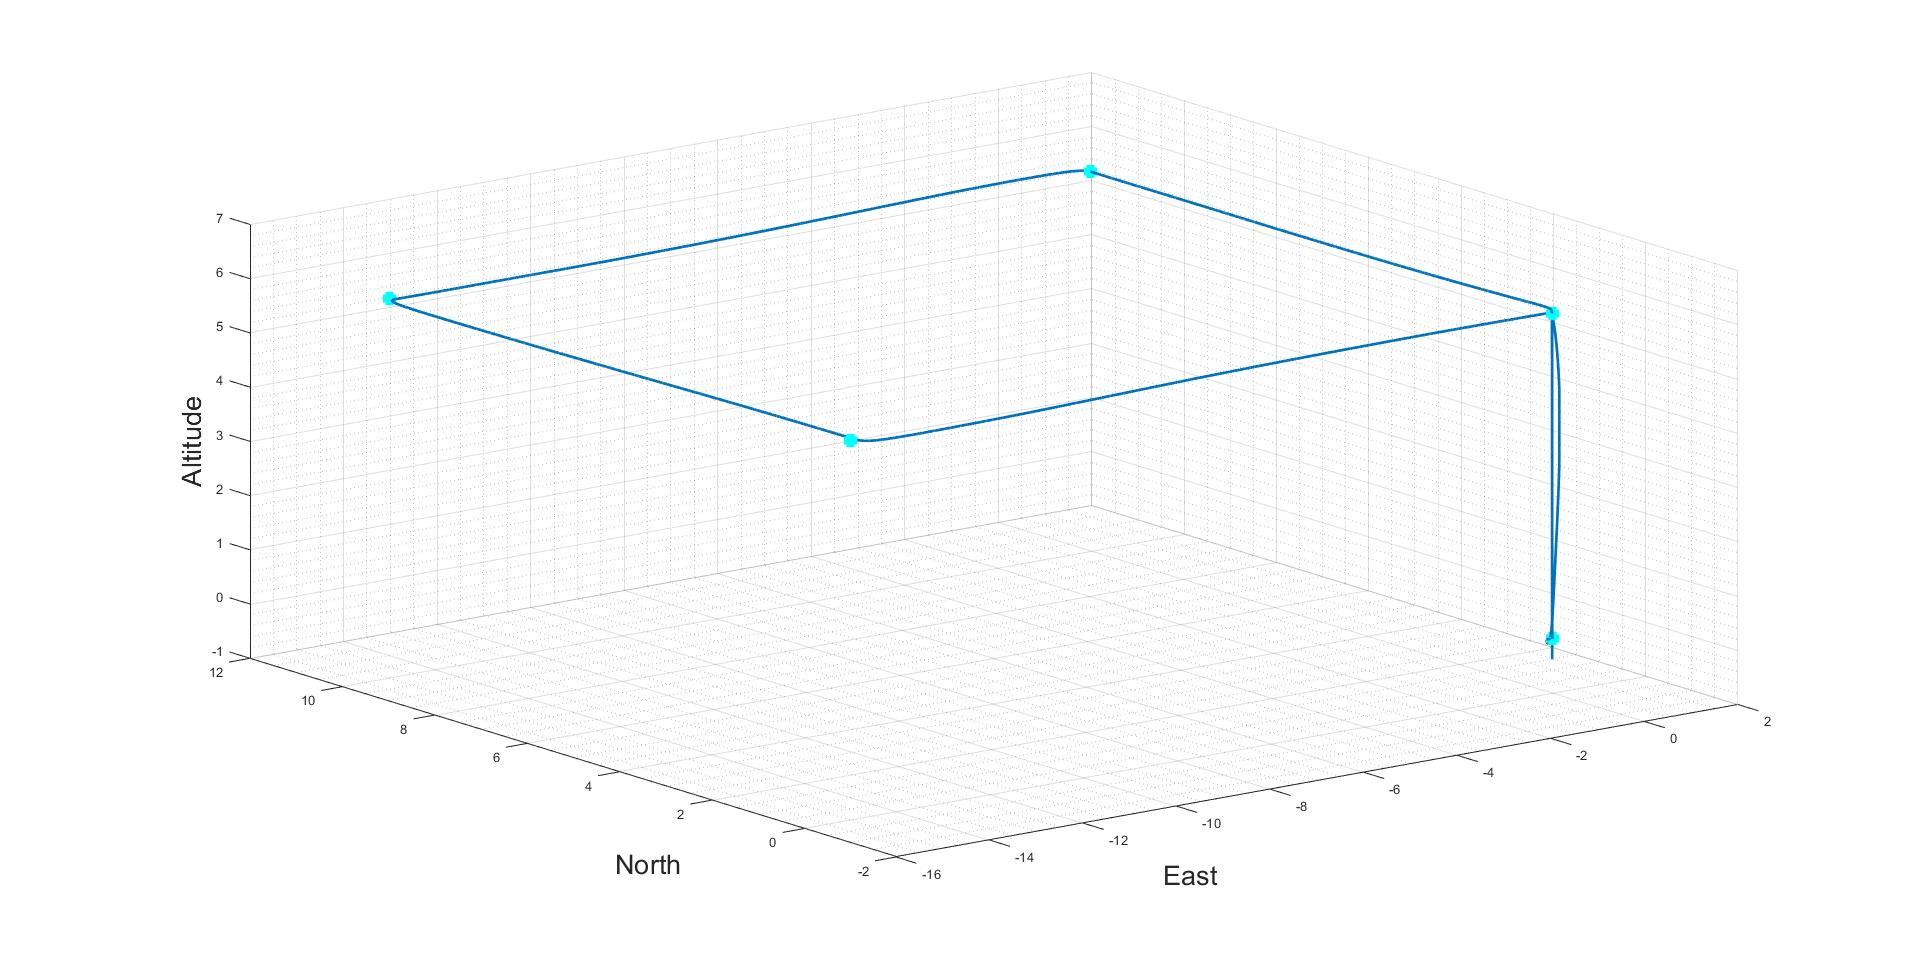
\includegraphics[height = 8.5cm]{../References/Diagrams/SimpleWaypointFlight.jpg}     
			\caption{Simple Waypoint Flight}
			\label{IM_WaypointFlight}
		\end{figure}
		
		\subsection{Yaw Alignment}
		The strategy for yaw alignment is to align the X-Axis of the drone's body frame with the current velocity vector. This achieves a constantly forward facing drone assisting in tight spaces as well as a more predictable sensor feedback for missions requiring additional sensors.
		
		The yaw angle controller designed in Section \ref{SSECT_YawAngleController} works on the basis of a yaw angle error. The heading alignment controller would be required to calculate a yaw error to be controlled by the yaw angle controller. Similarly to the tilt angle controller, this can be calculated using the dot and cross product between two vectors. The first vector is the current velocity in the body frame, while the second vector is the desired alignment vector. For alignment of the X-Axis the vector would be a unit vector containing only an X component. The X and Y components of the body velocity are extracted to calculate the magnitude of rotation where the axis of rotation should always be around the Z-Axis. The cross product is utilised to calculate the direction of the rotation. 
		
		\begin{figure}[H]
			\centering
			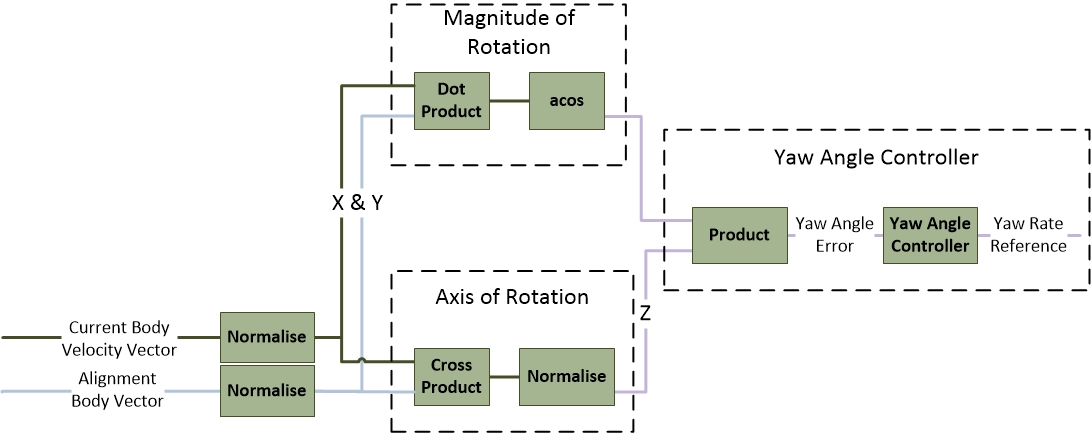
\includegraphics[height = 6cm]{../References/Diagrams/YawAlignmentController.jpg}     
			\caption{Yaw Alignment Controller}
			\label{IM_YawAlignmentController}
		\end{figure}
		
		\subsection{Yaw Alignment Discussion}
		At low speeds, while approaching position references, the proposed yaw alignment method can produce widely varying results. For this reason a minimum velocity magnitude is set, where below that limit the current yaw angle will be maintained. To demonstrate the effectiveness of the heading alignment, the drone is commanded to fly in a circle by commanding a North sine and East cosine velocity reference. Figure \ref{IM_YawAlignmentCircle} is the output from that experiment. The coloured line represents the current heading of the craft. As seen, the craft begins facing due North and as the craft starts to fly it's path, the craft follows and aligns itself accordingly.
		
		\begin{figure}[H]
			\centering
			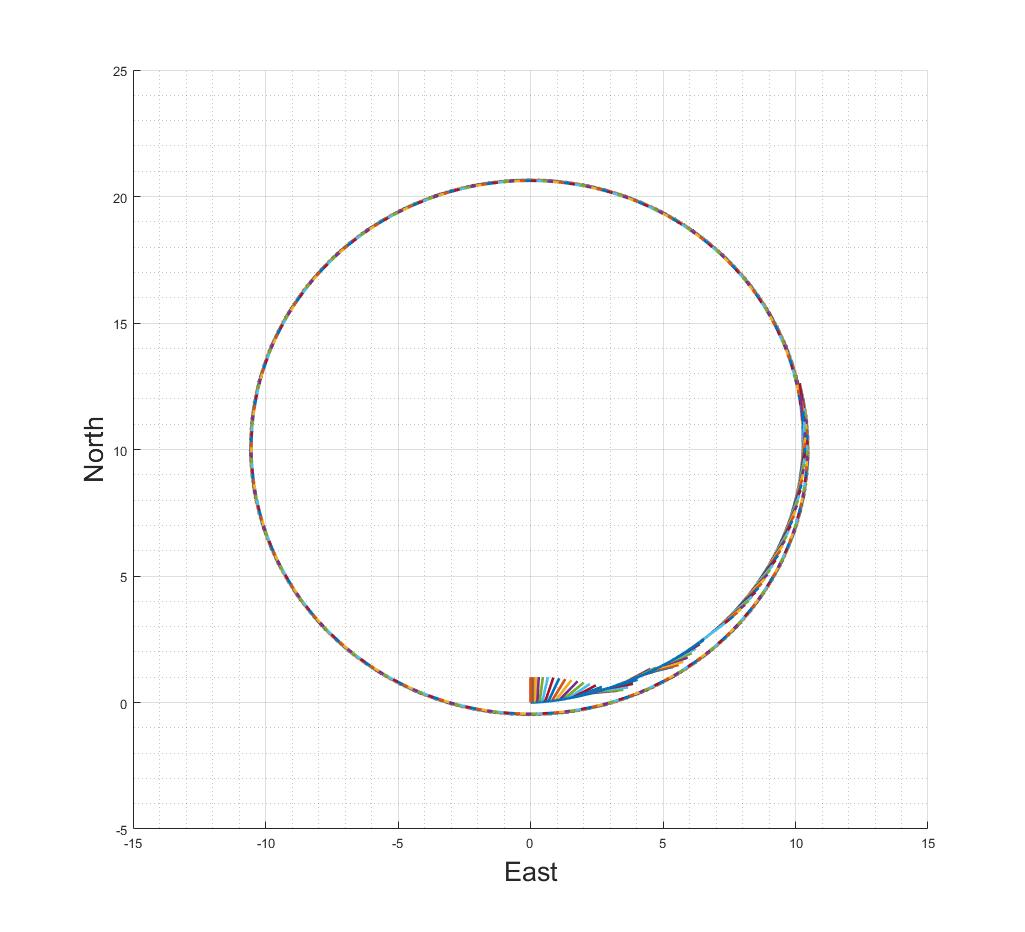
\includegraphics[height = 12cm]{../References/Diagrams/YawAlignmentCirc.jpg}     
			\caption{Yaw Alignment Controller}
			\label{IM_YawAlignmentCircle}
		\end{figure}
		
		Figure \ref{IM_YawAlignmentError} shows the calculated yaw angle error. As seen there is some initial overshoot, but the craft quickly settles onto the direct heading of the craft and maintains a close to zero yaw angle error.
		
		\begin{figure}[H]
			\centering
			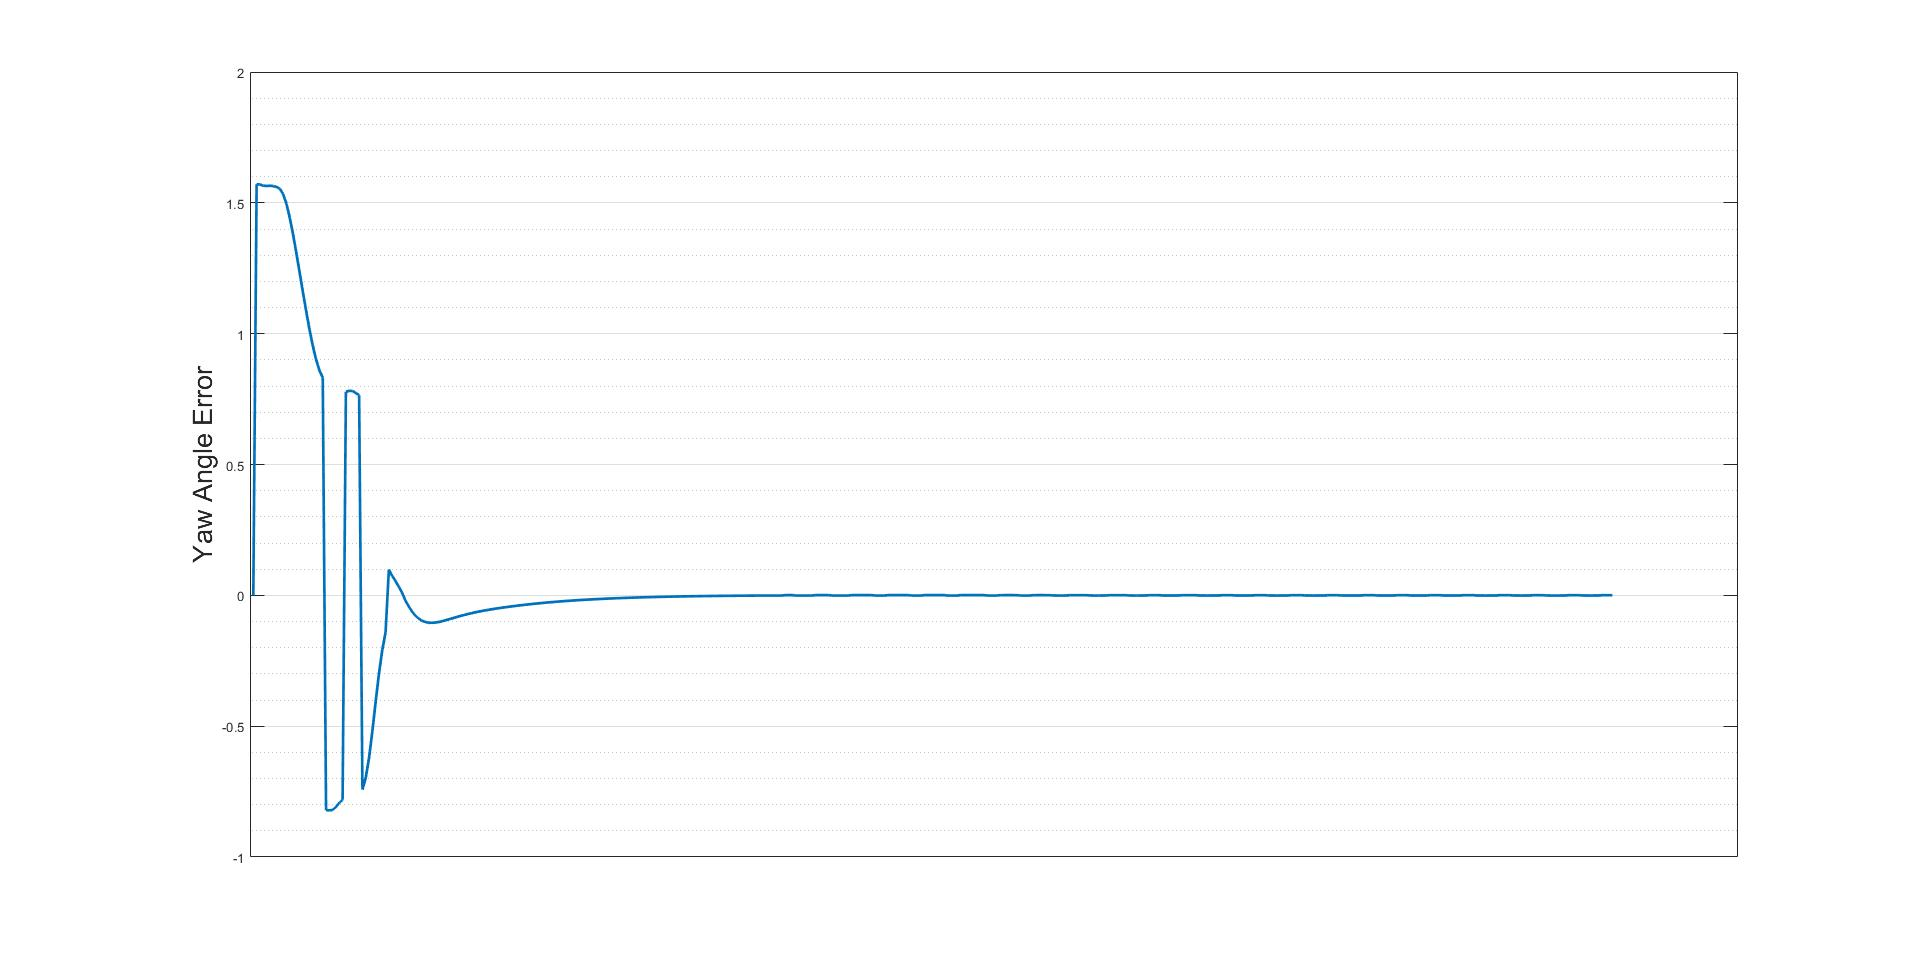
\includegraphics[height = 8cm]{../References/Diagrams/YawAngleError.jpg}     
			\caption{Yaw Angle Error}
			\label{IM_YawAlignmentError}
		\end{figure}
		
	\section{Obstacle Avoidance}
	The craft is required to navigate in an unknown environment without collision. The obstacle avoidance routine is responsible for ensuring the craft maintains a minimum set distance away from walls and other obstructions. When not in close proximity to any obstructions the obstacle avoidance routine should have a negligible effect on the craft which increases as the craft approaches a collision condition. Limited flight time dictates that the obstacle avoidance method should minimise deviation off of the desired path and allow the craft to reach the waypoints set by the waypoint generator when possible. The chosen obstacle avoidance controller should not affect the stability of the craft.
	
	The method will be based on proximity measurements generated by sensors on board the craft. To test and validate the implementation of the obstacle avoidance controller a mathematical model of the sensor feedback needs to be created.
	 
		\subsection{Mathematical modelling}
		Typical sensors used in this kind of application would be either ultrasonic proximity sensors, or in a high end application, a 360\textdegree\ laser range finder. This work assumes an ultrasonic sensor configuration and is modelled accordingly. 
		
		The proximity sensor placement is of critical importance to the functioning of the obstacle avoidance routine. The steps between proximity measurements are blind spots and can lead to the sensors missing an obstacle and subsequent crashing of the robot. Figure \ref{IM_SensorPlacement} shows the horizontal placement of sensors used in this work. There are eight sensors, all placed at 45\textdegree\, from each other. The vertical sensors used are placed in a simple up, down formation.
		
		\begin{figure}[H]
			\centering
			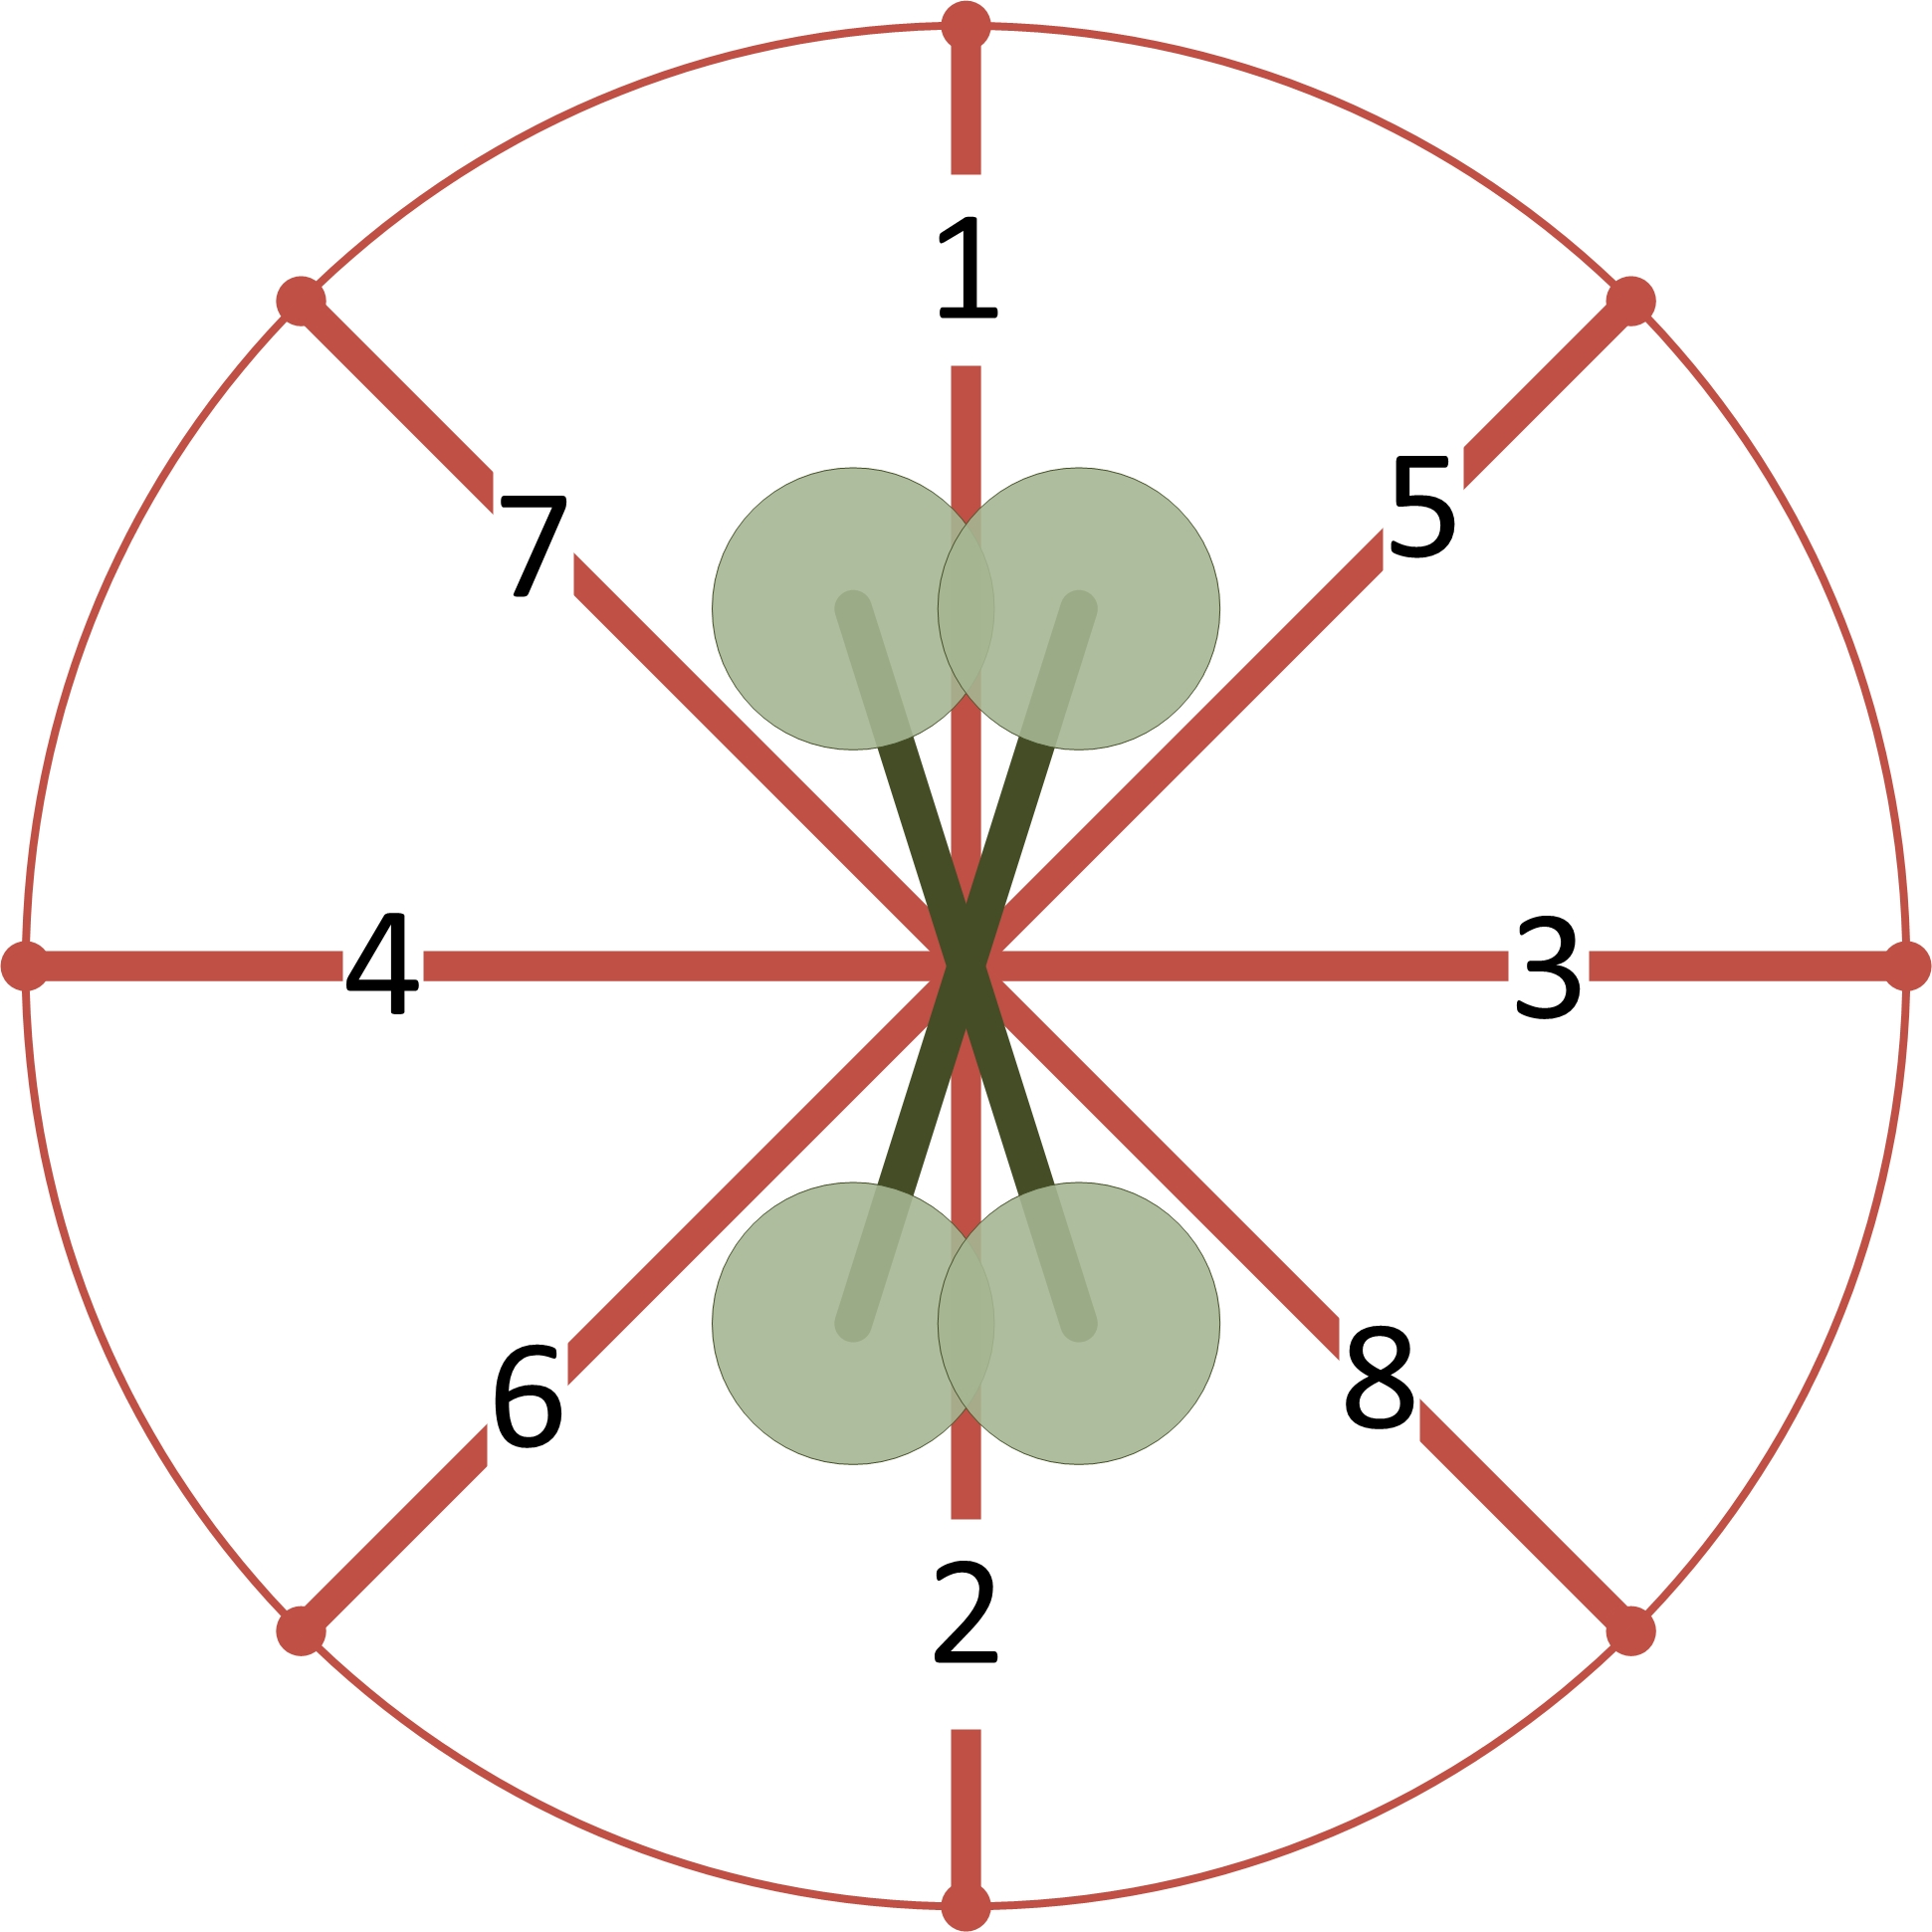
\includegraphics[height = 10cm]{../References/Diagrams/SensorPlacement.jpg}     
			\caption{Sensor Placement for Obstacle Avoidance}
			\label{IM_SensorPlacement}
		\end{figure}
		
		
		The measurements from ultrasonic sensors are subject to low amplitude, high frequency noise. Appropriate low pass digital filtering can be applied to the sensor by the data collection algorithm. There is still expected variations and errors in the sensor measurement due to uneven surfaces and large angles of deflection, corrupting the data from the sensors.
		
		Both the sensor arms and the environment are set up as a combination of straight line segments. The environment can be modelled as a complex combination of multiple line segments as shown by the outer blue lines in Figure \ref{IM_ObAvoidSetup}. For simplification, each vertical wall (walls existing in the North and East plane) is considered equal for all values of Down, and each horizontal wall (the roof and floor) is considered equal for each value of North and East. 
		
			\subsubsection{Obstacle Distance Detection}
			To calculate the distance measured by each sensor the model must successfully calculate the intersection of each sensor line segment, with each environment line segment. The vertical and the horizontal vectors are split up, allowing for the separate two dimensional calculation of horizontal intersections and the one dimensional calculation of vertical intersections.
			
			The two dimensional calculation is done using a well documented line segment intersection equation. A line segment is considered as a finite portion along a line, dictated by two points existing on that line. The equations of the line segments can be represented mathematically as shown in \eqref{EQ_LineSegment} - \eqref{EQ_LineSegment1}. $p_1$ and $p_2$ are the end and start points of the first line segment with $p_3$ and $p_4$ belonging to the second line segment. The equations of each line segment hold true for the case of $0 \leq t \leq 1$ expressing a position along the defined segment. 
			
			\begin{eqnarray}
			p_1 &=& t(p_2 - p_1) \label{EQ_LineSegment}\\\label{EQ_LineSegment2}
			p_3 &=& t(p_4 - p_3) \label{EQ_LineSegment1}
			\end{eqnarray}
			
			The definition of an intersection is where these two lines are equal, breaking the equation into x and y components then creates equations \eqref{EQ_Intersect} - \eqref{EQ_Intersect1}. Where $t_a$ and $t_b$ are the offsets for each respective line segment.
			
			\begin{eqnarray}
			x_1 + t_a(x_2 - x_1) &=& x_3 + t_b(x_4 - x_3) \label{EQ_Intersect}\\\label{EQ_Intersect2}
			y_1 + t_a(y_2 - y_1) &=& y_3 + t_b(y_4 - y_3)) \label{EQ_Intersect1}
			\end{eqnarray}
			
			The final step is to solve for both $t_a$ and $t_b$. If both $t_a$ and $t_b$ exist between 0 and 1, then it is known that the line segments intersect. If either $t_a$ or $t_b$ exist outside of this range then the general lines intersect outside of the described segment constraints. If the lines are collinear, no intersection of the general lines, the result for $t_a$ and $t_b$ will be unsolvable. There might exist a possibility where the sensor line segments intersect with multiple walls, in this case the sensor would only return the closest obstacle. As mentioned, distance measurement devices struggle to return accurate results when the angle between the object and the sensor is very large. In this case the intersection is not recorded as to mimic a realistic sensor. In the case that no intersection is measured, the sensor would return it's maximum range.
			
			Figure \ref{IM_ObAvoidSetup} shows the typical result of a single obstacle detection frame. The red dots show the calculated intersection between the sensor arms and the environment. The corresponding distances are summed into a single proximity vector with the negative of that vector representing an obstacle avoidance vector shown in cyan. 
			
			\begin{figure}[H]
				\centering
				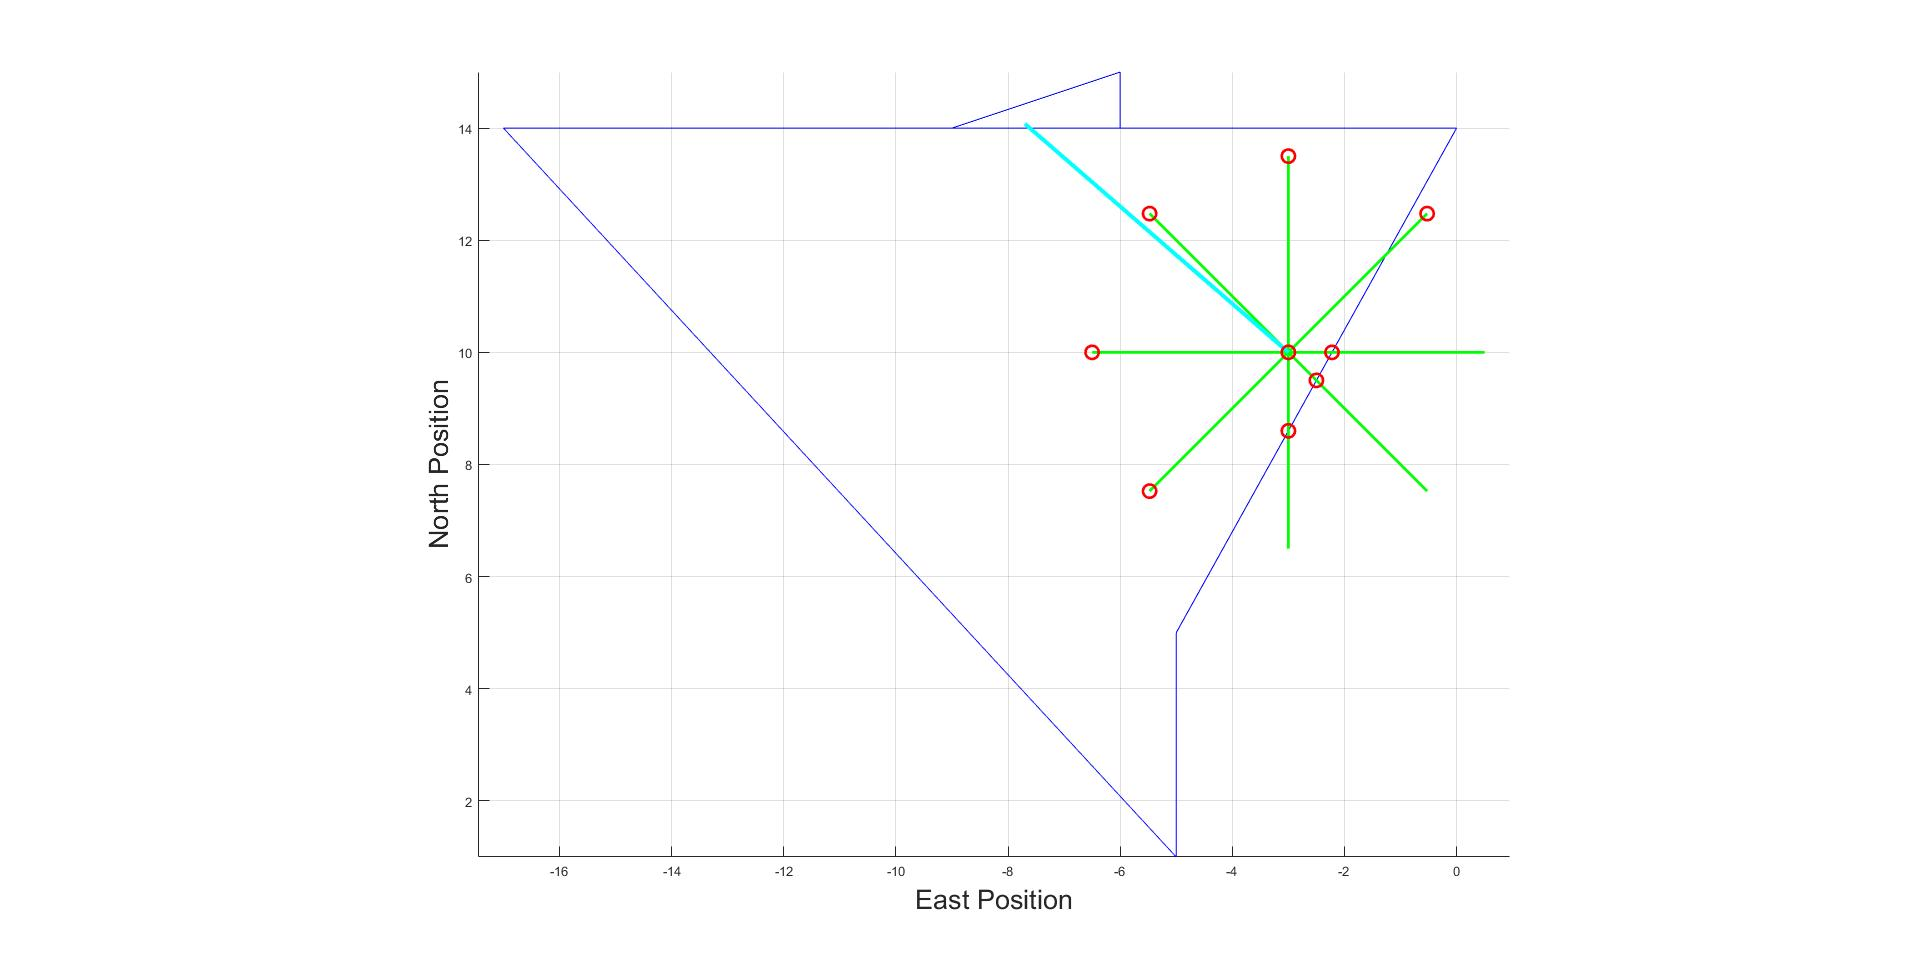
\includegraphics[height = 8.5cm]{../References/Diagrams/ObAvoidDemo.jpg}     
				\caption{Obstacle Detection Demonstration}
				\label{IM_ObAvoidSetup}
			\end{figure}
	
		\subsection{Obstacle Avoidance Methodology}
		The requirements for the obstacle avoidance routine are discussed above while different methodologies for collision avoidance were investigated in Section \ref{ObAvoidLit}. This section begins by discussing these methods and how the conclusions for the chosen method were made based on the requirements for this work. The section is concluded by explaining the final implementation and it's controller.
		
			\subsubsection{Methodology Investigation}
			Three methods were explored to make an informed decision on the final implementation of the obstacle avoidance method. 
			
			The Bug algorithm will create a new path for the craft to follow based on local scans of an environment. This deviation off the set path could be useful when the craft is required to perform exploratory missions inside unknown environments, allowing the vehicle to traverse a walls contour until it finds the appropriate path again. However, the contours and new paths can lead the craft to deviate far off the desired path. 
			
			The potential field method utilises both the attractive potential of the target and the repelling forces of obstacles. The use of immediate distances from the craft limits the requirement for constant scanning and replanning of the route. This method will allow the craft to deviate off a given path while still maintaining an attractive potential to the end target. The position controller creates an attractive potential by commanding velocities proportional to distance error from a target. The obstacle avoidance routine will then need to apply it's repelling potential as a velocity command as well. The potential field method also allows for relationships other than linear with the distance from the craft. The repelling potential could be generated from a quadratic, or even higher order polynomial, relationship with distance.
			
			The last considered method is to utilise the benefits of a spring damper system. Using the maximum sensor distance as the resting distance, a virtual spring and damper can be created as depicted in Figure \ref{IM_SpringDamper}.
			
			\begin{figure}[H]
				\centering
				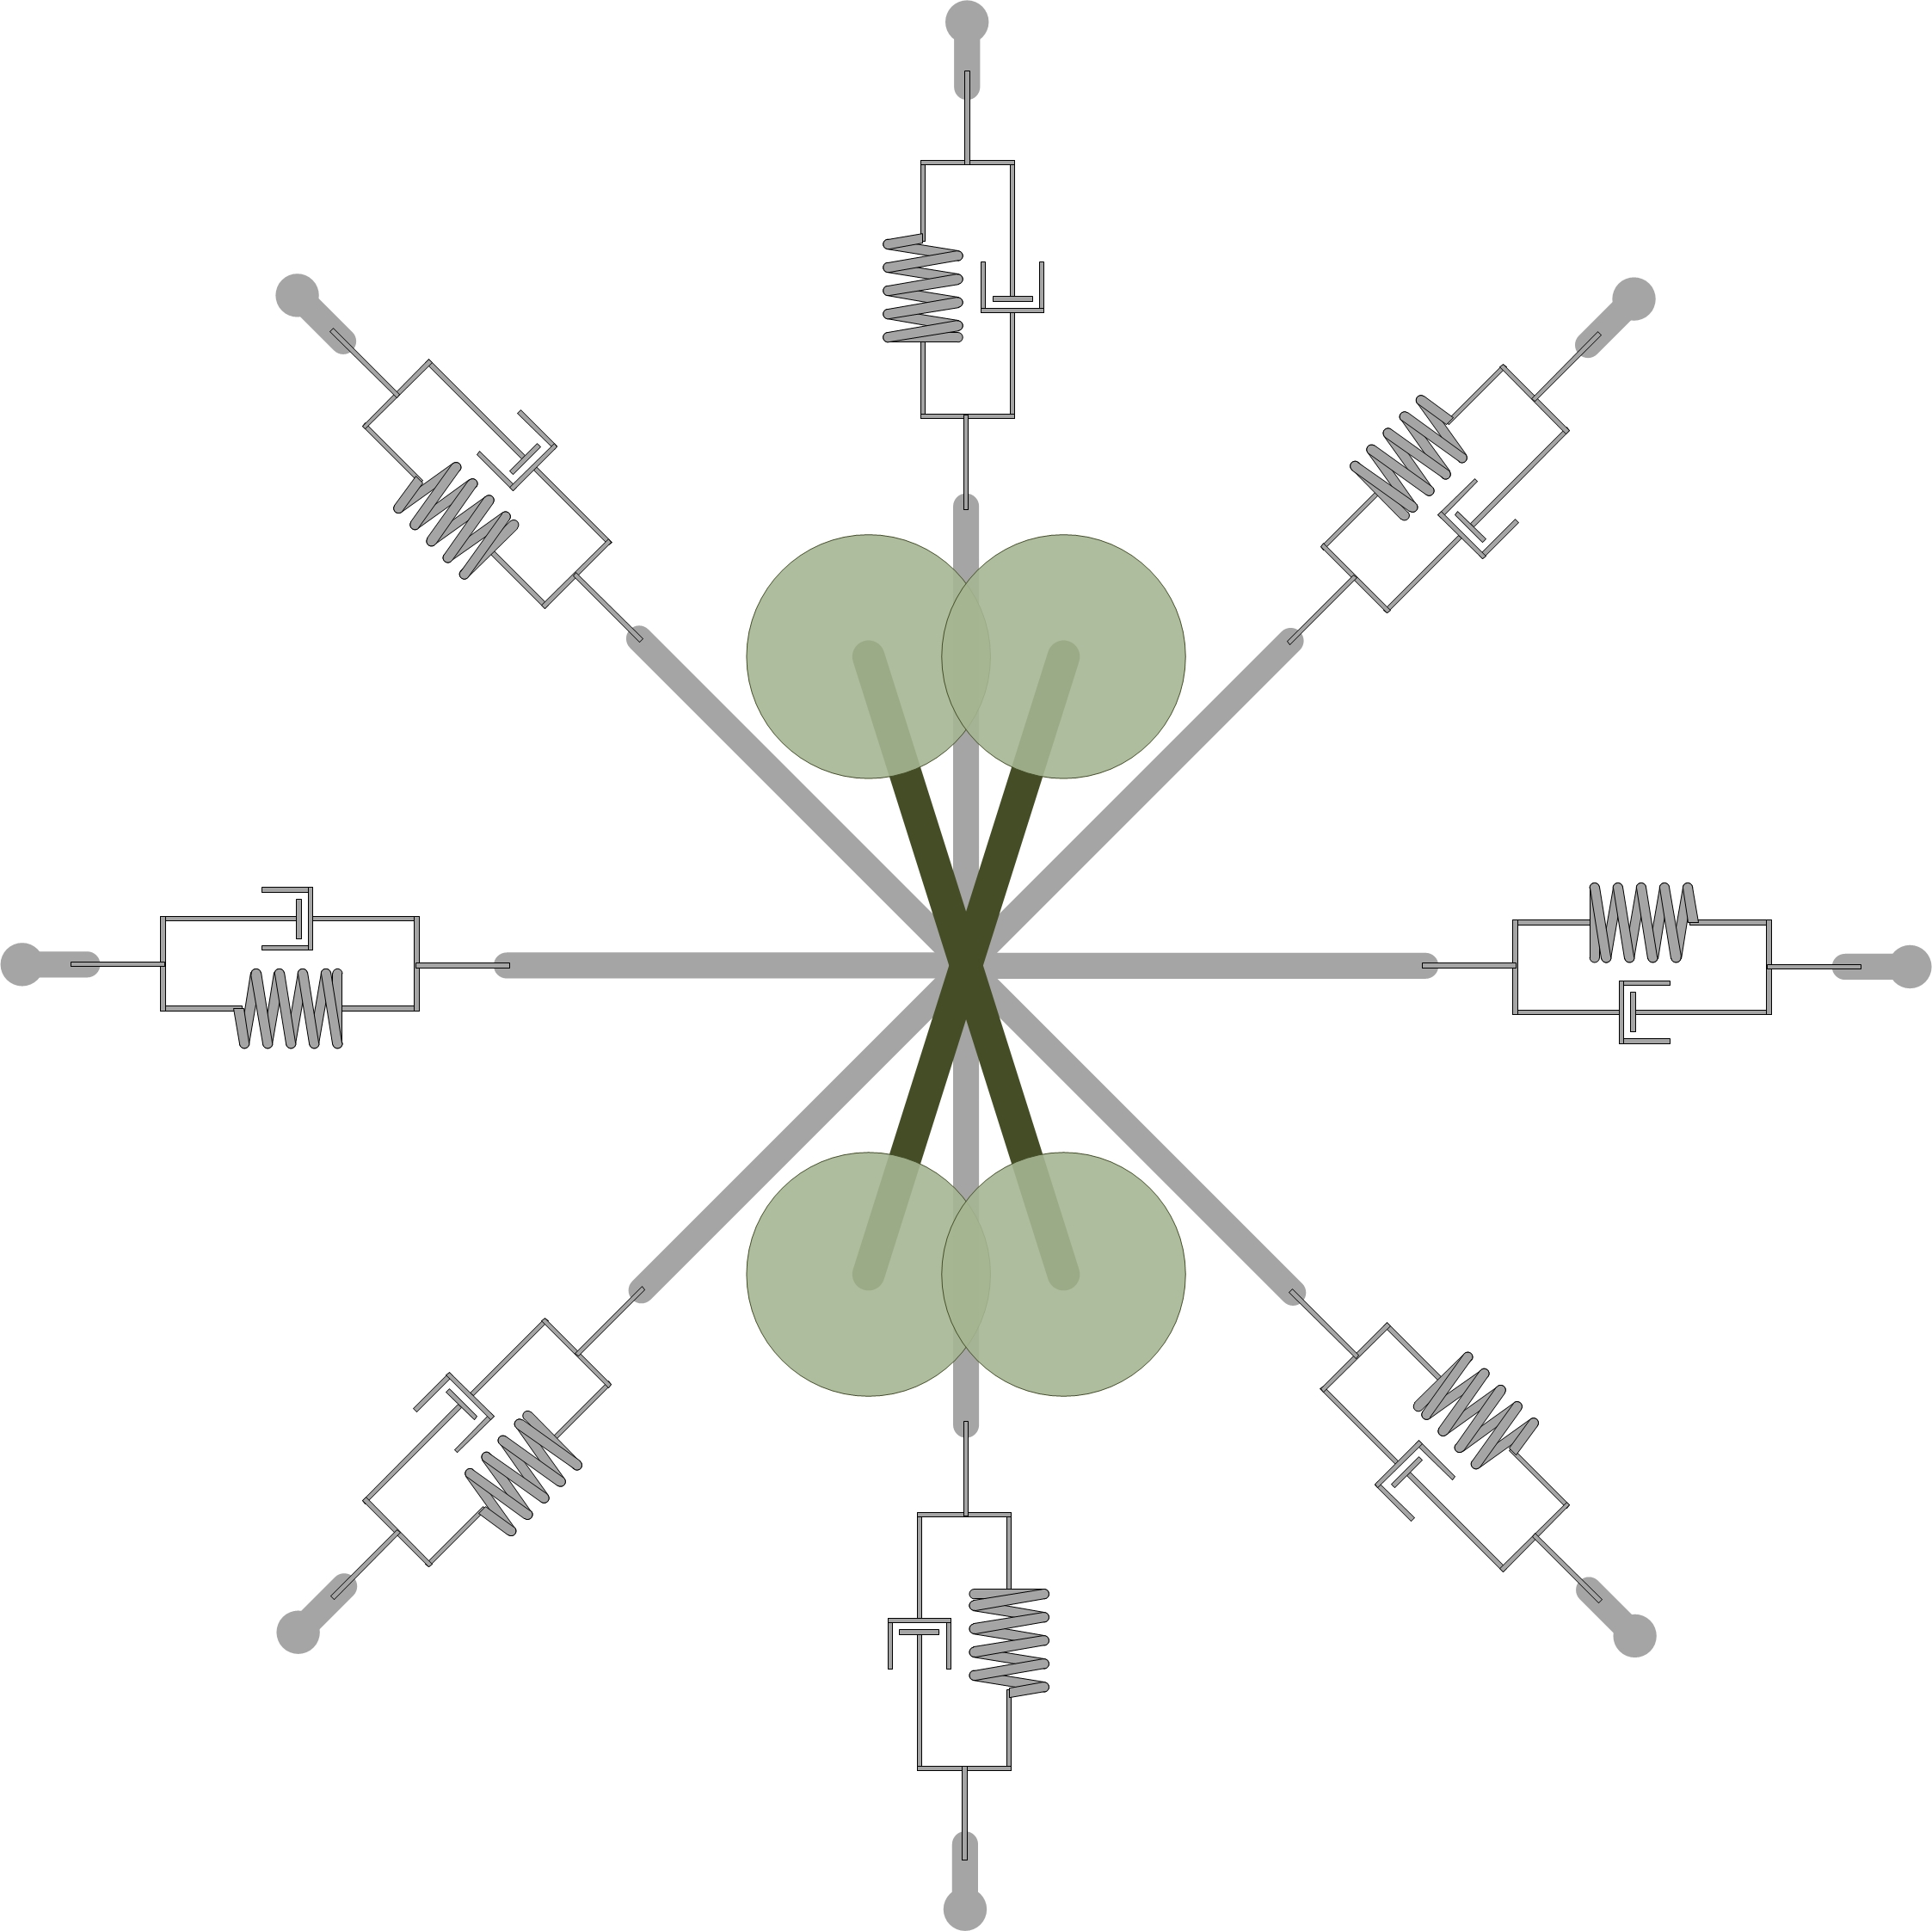
\includegraphics[height = 10cm]{../References/Diagrams/SpringDamper.jpg}     
				\caption{Visual descriptive aid for a virtual spring damper sensor system}
				\label{IM_SpringDamper}
			\end{figure}
					
			The spring force can be used to push the drone away, but should not pull the vehicle towards an obstacle. The forces created by the spring should be added directly to the acceleration commands creating a virtual force. The damper is added to reduce the oscillations caused by the spring as it comes in and out of contact with the wall. The location of the spring damper in the inner control loops ensures a fast acting system, but requires a high bandwidth. The horizontal velocity controller's lag compensators also adds additional dynamics to the system that the obstacle avoidance system will need too interact with.
			
			Each method has benefits and potential hindrances. The next section discusses combining these methods to form a successful obstacle avoidance implementation.
			
			\subsubsection{Methodology Implementation}
		
			This section describes the methodology behind the chosen obstacle avoidance routine. The system works on the basis of the potential field method investigated in Section \ref{SSECT_PotentialField}. Figure \ref{IM_ObAvoidController} demonstrates how the controller feeds into the existing overall controller structure. As shown, the obstacle avoidance controller subtracts from the position controller's velocity set point to create a new velocity set point. Both set points are limited before being subtracted from one another. To ensure that the obstacle avoidance takes control to avoid collisions, the position controller is limited to a smaller value than that of the obstacle avoidance controller.
			
			\begin{figure}[H]
				\centering
				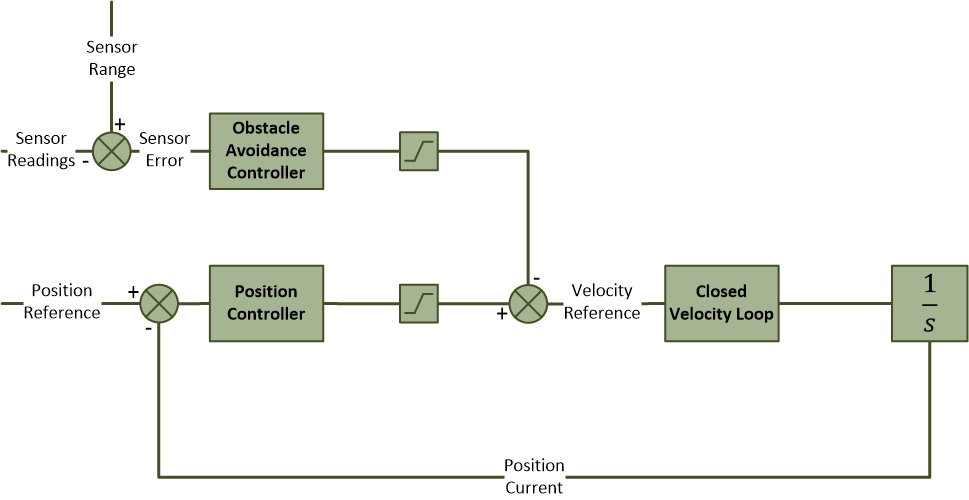
\includegraphics[height = 6cm]{../References/Diagrams/ObstacleAvoidanceController.jpg}     
				\caption{High level view of obstacle avoidance controller}
				\label{IM_ObAvoidController}
			\end{figure}
			
			The sensor values are all used and summed together to create an obstacle avoidance vector. This provides abstraction to the actual sensor placement used in practise. As long as the angle of each sensor is known a single vector can be created and used in the obstacle avoidance controller. To mimic the existing position controller structure a North, East and Down velocity command are created.
		
			\subsubsection{Obstacle Avoidance Controller}
			As shown in Figure \ref{IM_ObAvoidController}, the obstacle avoidance controller generates a velocity setpoint reference and works in conjunction with the existing position controller. A 3-axis stable position controller has been designed in the controller chapter. The allowed gain and bandwidth of the obstacle avoidance controller can be inferred from the gain calculated for the existing controller. The sensor error is calculated by subtracting the current sensor measurement from the maximum sensor range and squaring the result. This quadratic relationship causes the obstacle avoidance controller to have a large effect when close to obstacles and less of an effect when obstacles first come into measuring distance. 
			To limit the oscillations when approaching a wall, a derivative controller component is added. This component is calculated by taking the velocity along each sensor arm and applying a gain to each calculated velocity. It must be ensured that the derivative controller component is only active when the specific sensor is in measurement range. Figure \ref{IM_SensorController} shows the implementation of the controller.
			
			\begin{figure}[H]
				\centering
				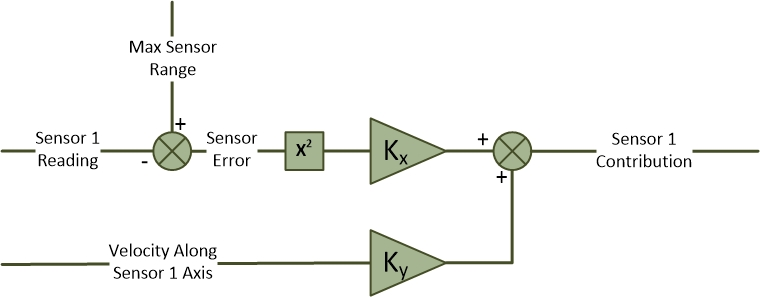
\includegraphics[height = 6cm]{../References/Diagrams/SensorController.jpg}     
				\caption{Individual Sensor Controller}
				\label{IM_SensorController}
			\end{figure}
			
			The controller attempts to drive each of the combined contributions to zero. This condition is met when there are no obstacles, or when all opposing sensors measure the same result, maintaining a equilateral distance from each wall. Figure \ref{IM_SensorCombination} shows how each sensor is combined. The sensor naming convention seen is specified in Figure \ref{IM_SensorPlacement}.
			
			
			A final consideration is the arm length of the sensor. The sensor maximum range should allow the craft to fly with none of the sensors active, but should also provide enough time for the system to respond. The gain of the controller should be considered at worst case, this occurs when the sensor is at a distance of close to zero, creating a sensor error equal to the square of the maximum sensor distance. To maintain stable system it is intuitive that the $K_x$ gain of the sensor controller will decrease quadratically as the arm length increases. An arm length range of $2.5$\,m - $4$\,m was decided. Increasing the derivative gain increase the total damping in the system allowing for a higher $K_x$ gain.
			
			The selection of the saturations, arm length and gains will decide how close the craft will be allowed to a given obstacle. 
			
			\begin{figure}[H]
				\centering
				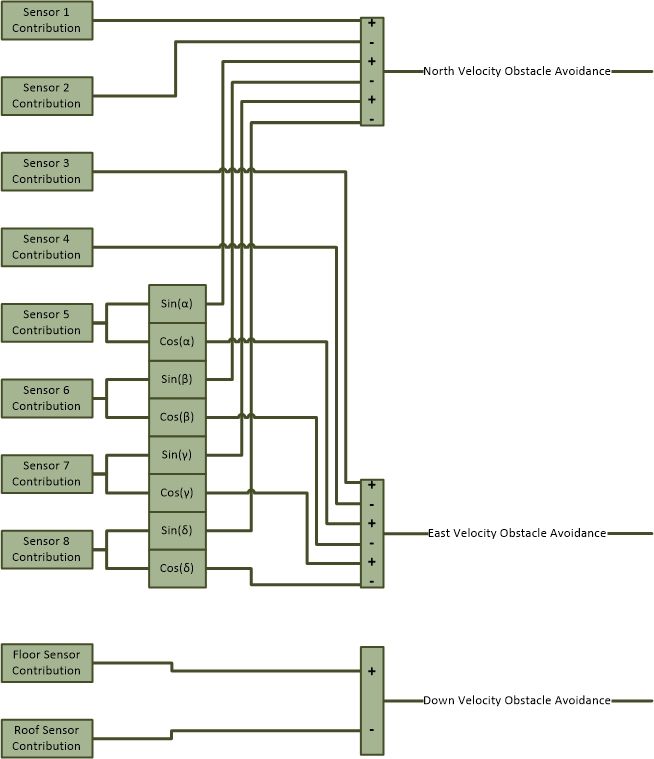
\includegraphics[height = 16cm]{../References/Diagrams/SensorCombination.jpg}     
				\caption{Sensor Combination}
				\label{IM_SensorCombination}
			\end{figure}
			

				
		\subsection{Obstacle Avoidance Discussion}
		The discussion is required to assess the feasibility and stability of the proposed obstacle avoidance routine. A simple method to assess this is by disabling the position controller and allowing the obstacle avoidance routine complete control of the aircraft's velocity reference commands. To create this scenario wall segments are placed at $-0.5m$ and $4m$ North and East, with a floor at $0m$ and roof at $-6m$ Down. The horizontal sensor range is set at $3.5m$ with the vertical sensor range set to $2m$. The craft is started at position (0, 0, 0), in the bottom left corner of the four walled room.
		
		The images shown in Figure \ref{IM_ObAvoidPos} show the North, East and Down position respectively of the craft as it is controlled by the obstacle avoidance controller. The images on the right show the velocity set points sent by the controller to the inner velocity loop. As shown the craft is stable and moves steadily to the centre of the room with the velocity commands tending towards zero. 
		
		\begin{figure}[H]
			\begin{tabular}{c c}
				\centering
				{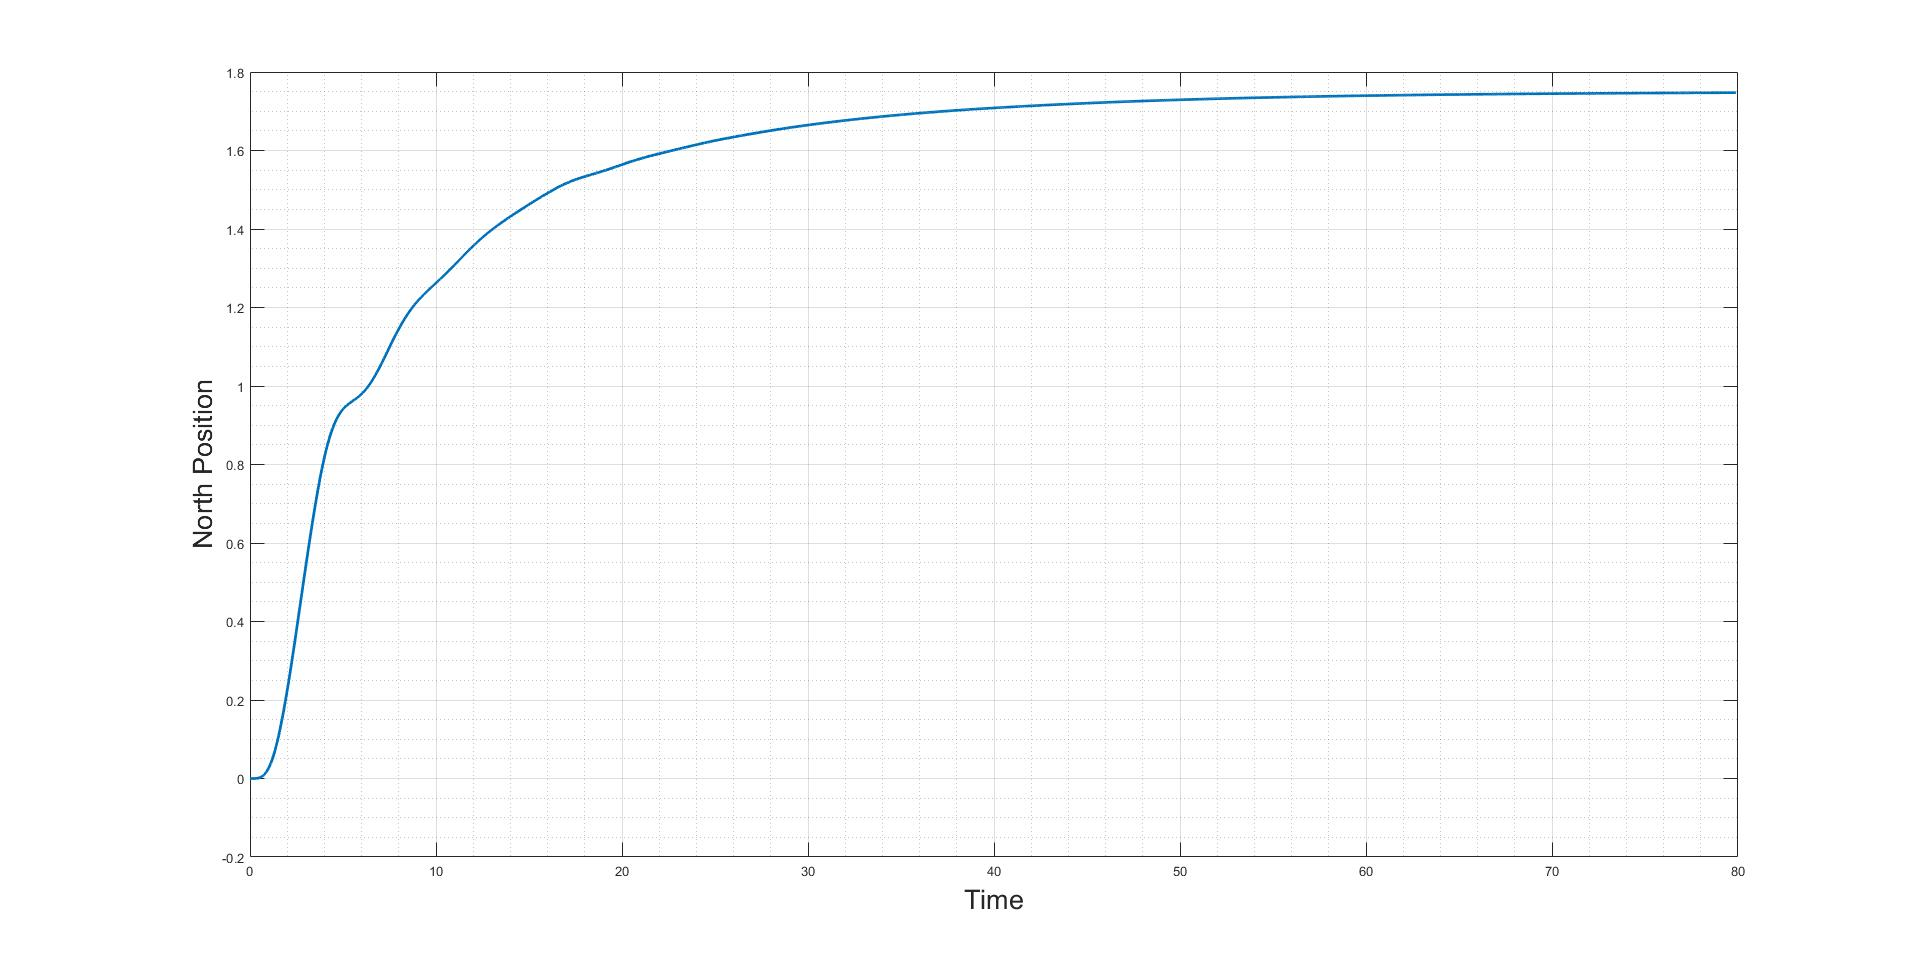
\includegraphics[width = 3in]{../References/Diagrams/ObAvoidNorth.jpg}} &
				{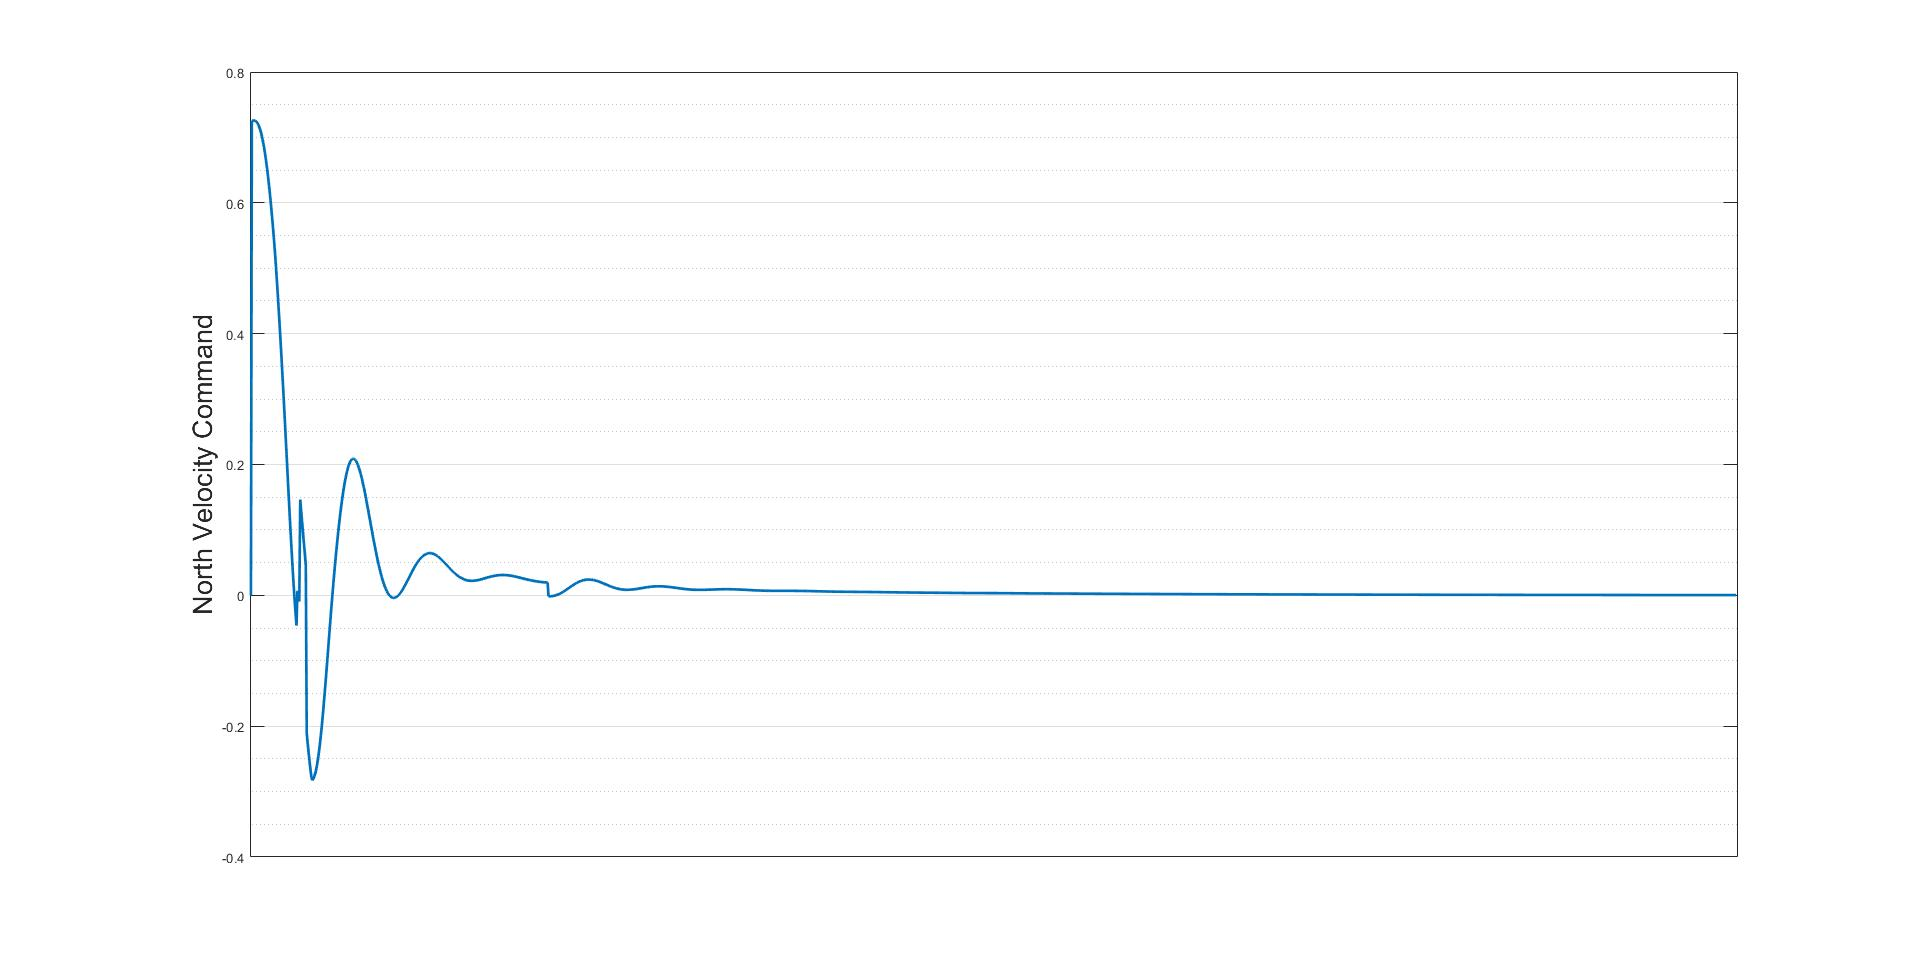
\includegraphics[width = 3in]{../References/Diagrams/ObAvoidVelNorth.jpg}}\\
				{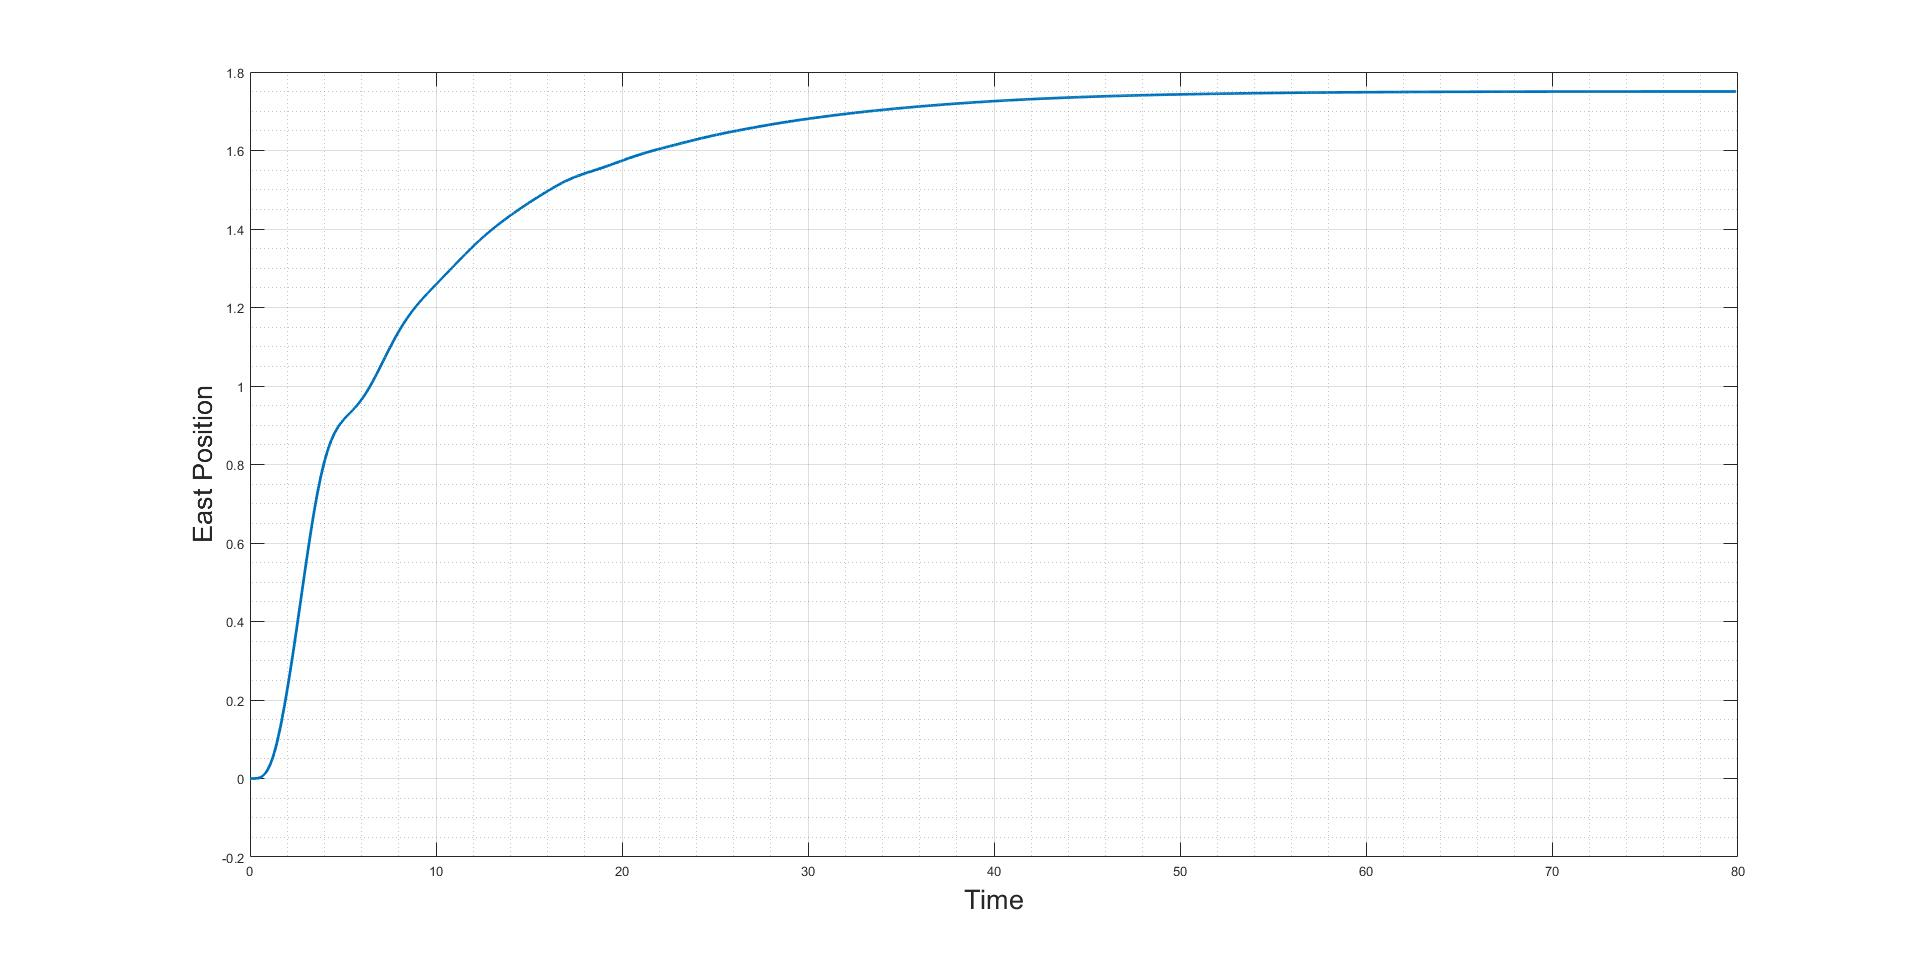
\includegraphics[width = 3in]{../References/Diagrams/ObAvoidEast.jpg}} &
				{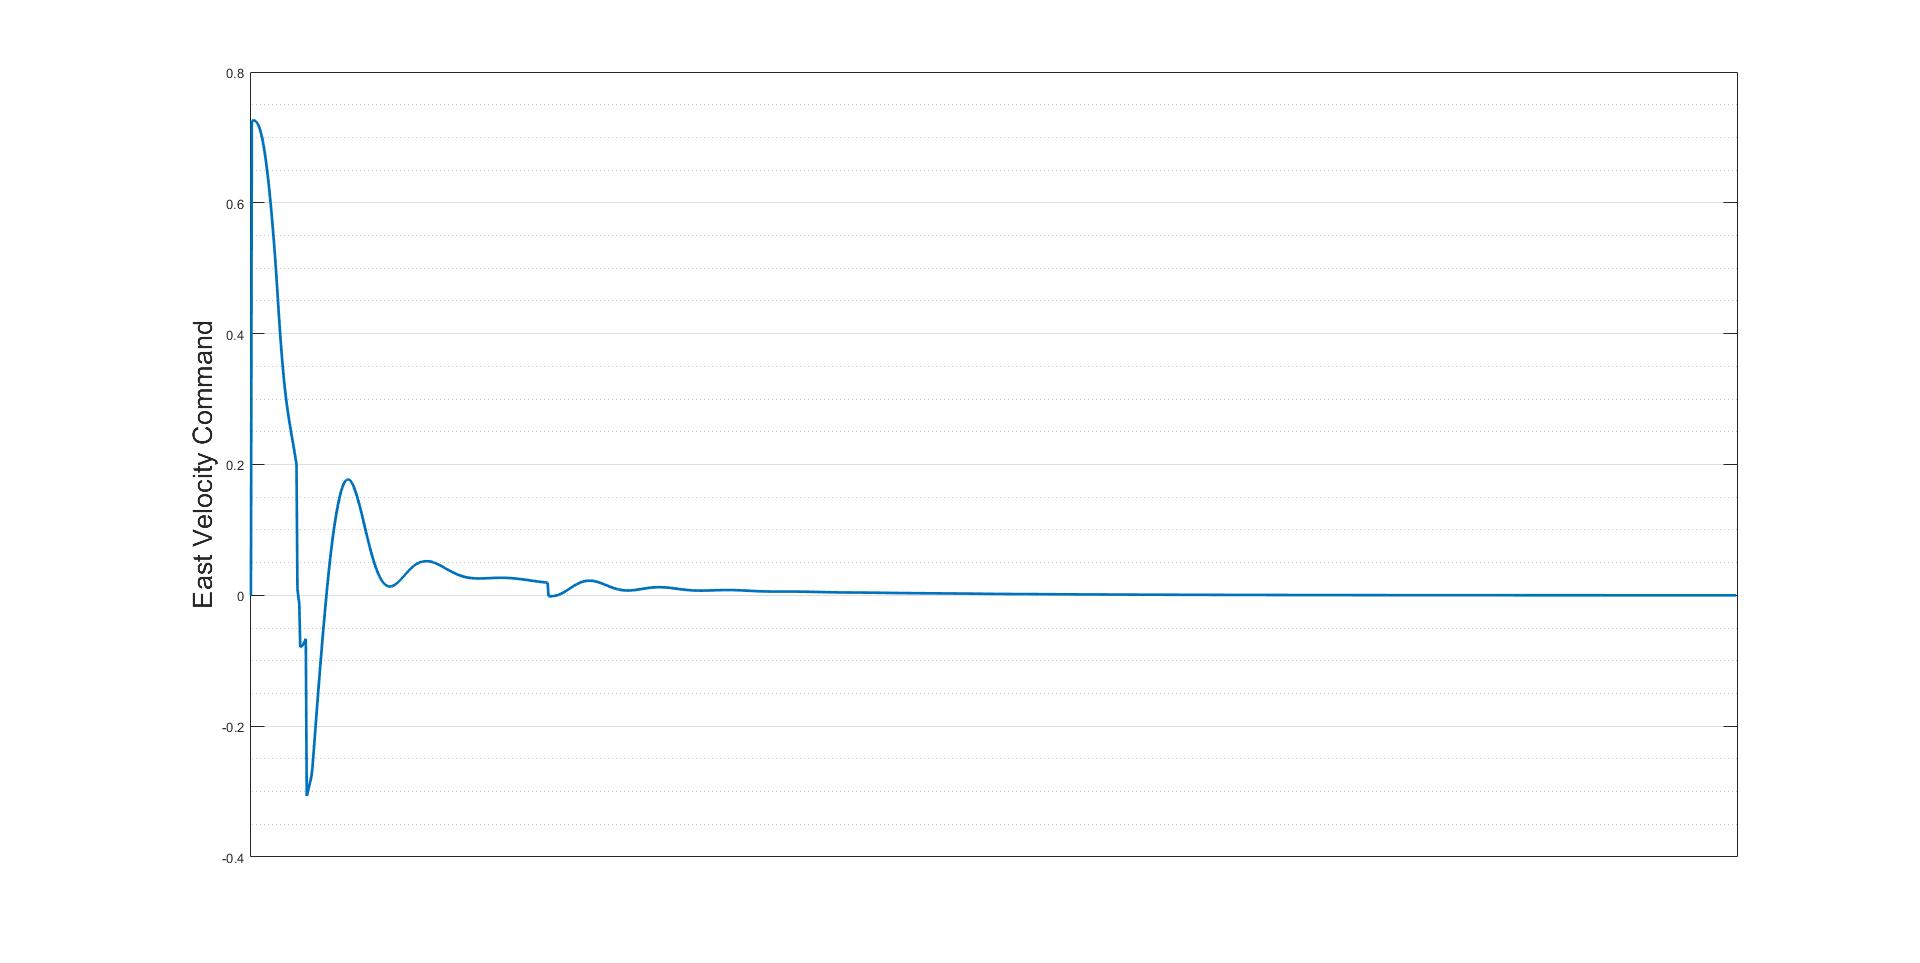
\includegraphics[width = 3in]{../References/Diagrams/ObAvoidVelEast.jpg}}\\
				{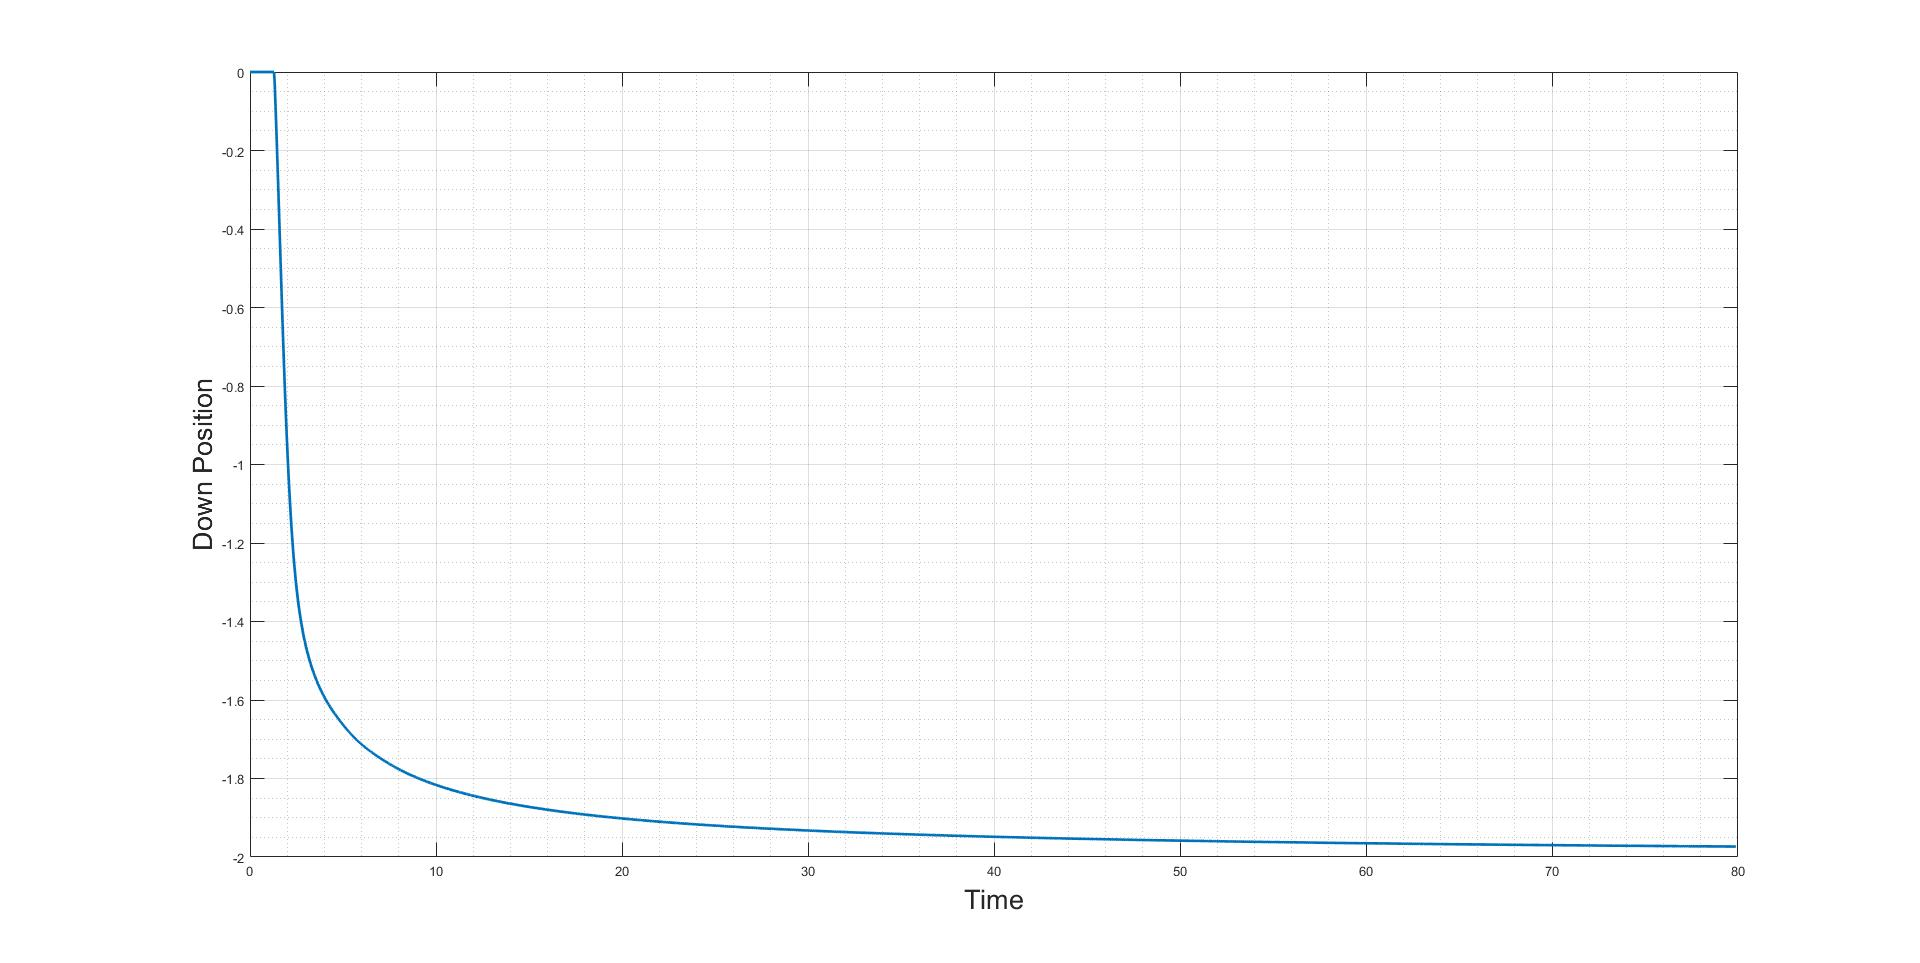
\includegraphics[width = 3in]{../References/Diagrams/ObAvoidDown.jpg}} &
				{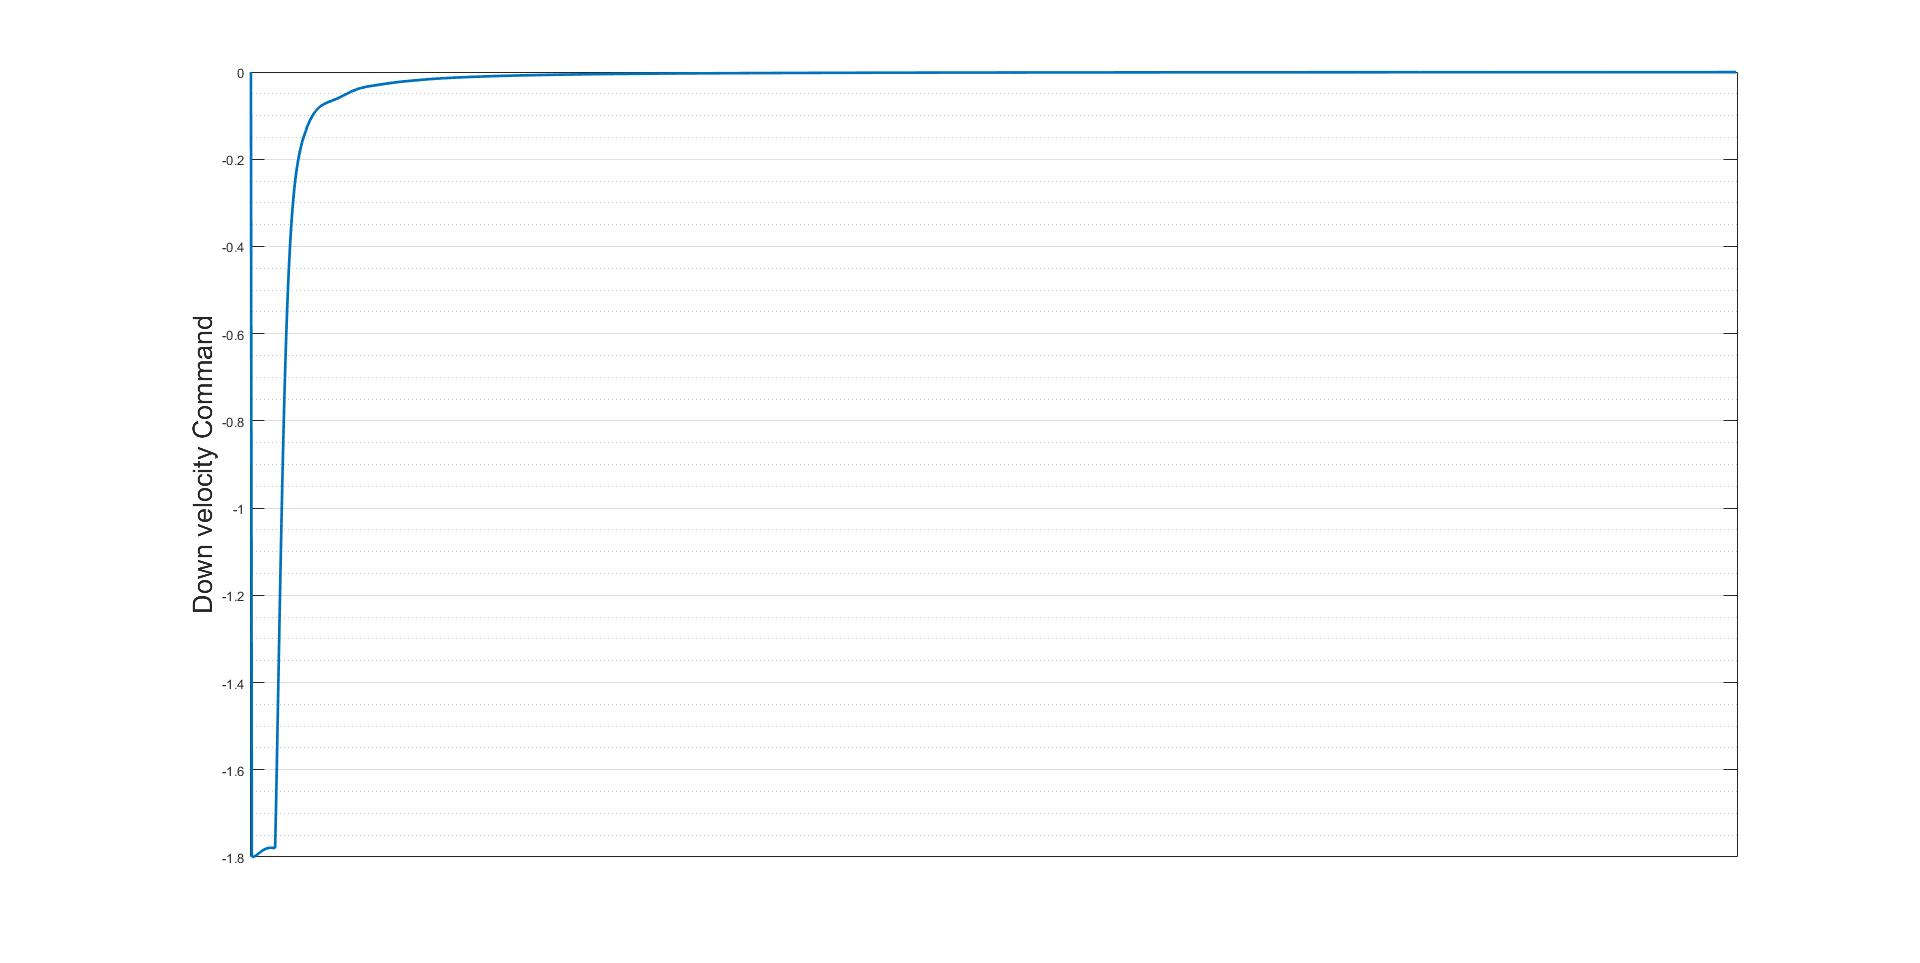
\includegraphics[width = 3in]{../References/Diagrams/ObAvoidVelDown.jpg}}
			\end{tabular}
			\caption{Position control using only the obstacle avoidance controller (Position (Left), Velocity Command (Right), North (Top) East (Middle), Down (Bottom))}
			\label{IM_ObAvoidPos}
		\end{figure}
	
		To demonstrate the interaction of the obstacle avoidance routine with the position controller a wall is set up at $10$\,m and the craft is commanded to go to $17$\,m. This test will ensure that the obstacle avoidance controller works when the craft is travelling at maximum speed. Figure \ref{IM_ObAvoidTest1} shows the North position of the craft in blue, the commanded position in red and the dotted line represents the position of the wall. As seen, the craft stops within $0.5$\,m of the wall.
		
		\begin{figure}[H]
			\centering
			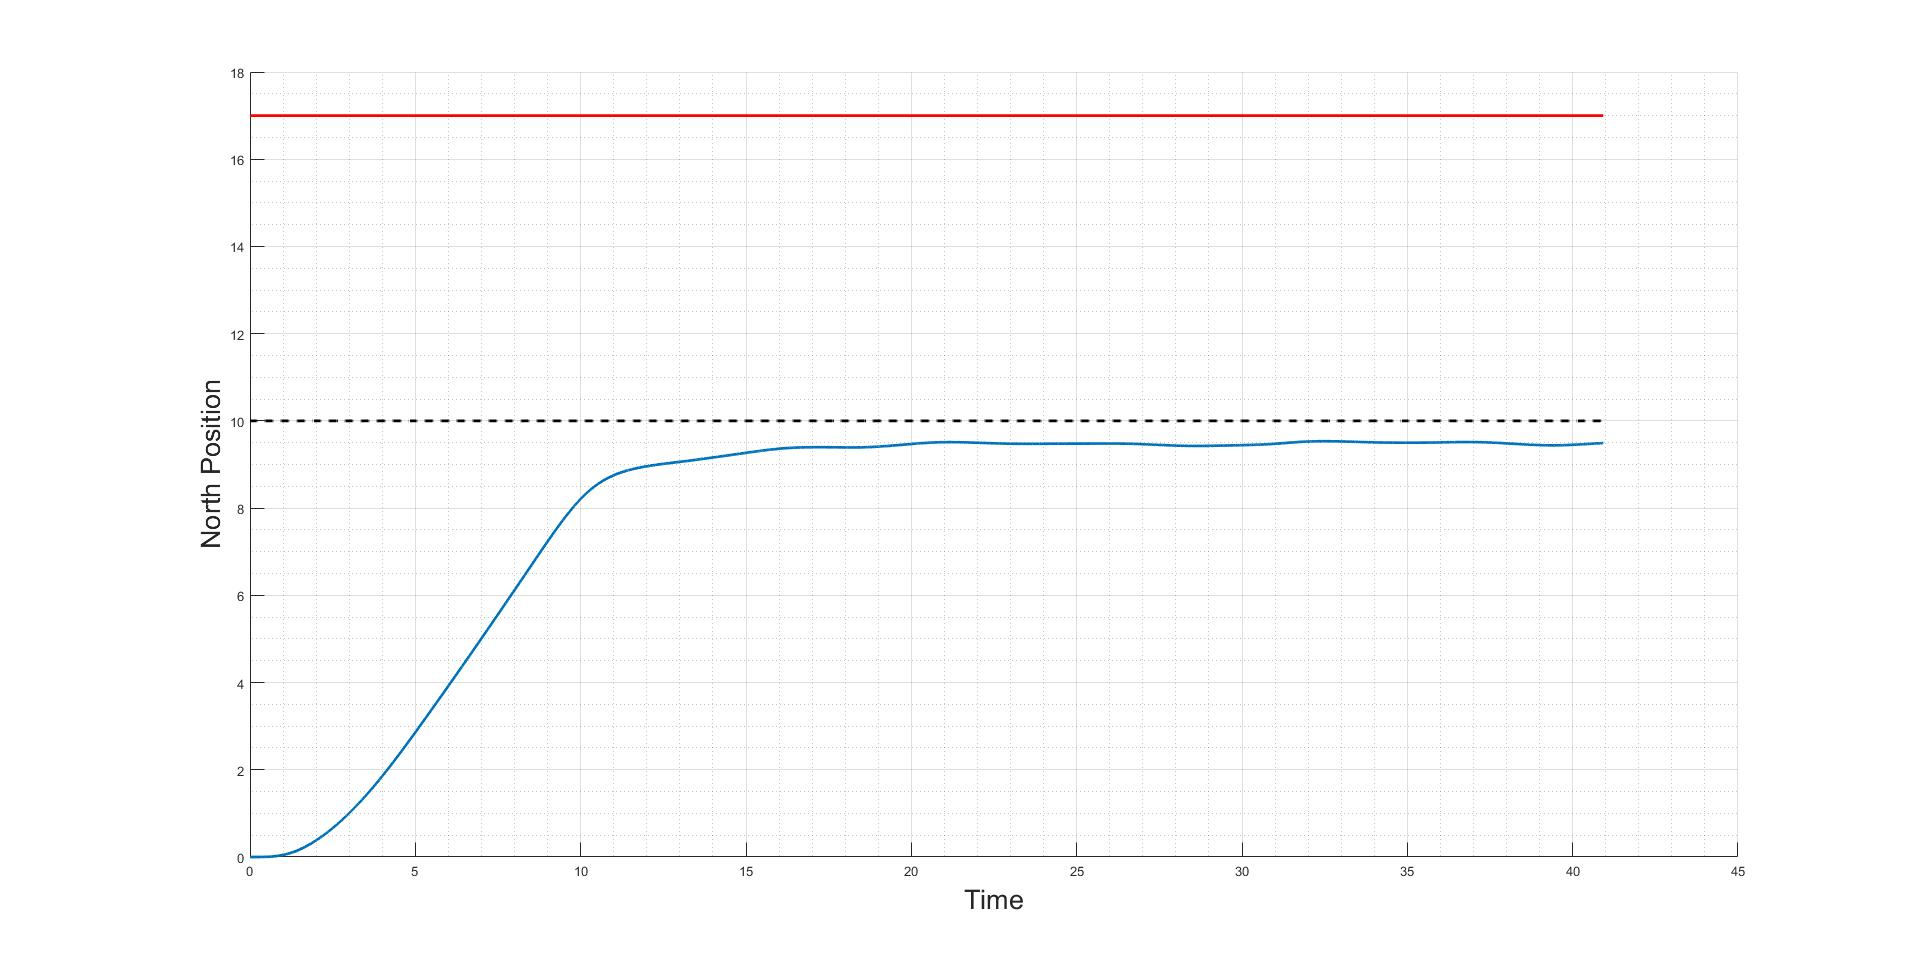
\includegraphics[height = 8cm]{../References/Testing/ObAvoidStraightWallNorth.jpg}     
			\caption{Sensor Combination}
			\label{IM_ObAvoidTest1}
		\end{figure}
					
		Although these examples show the method as an effective means of obstacle avoidance, this method has limitations that are explored in the proceeding flight tests chapter.
		
			